% Vietnamese translation for OI Public Library
% Source-PDF: IOI中国国家候选队论文/2004/汪汀.pdf
\documentclass[11pt]{article}
\usepackage{oipl-vn}
\usepackage{tikz}
\usetikzlibrary{arrows.meta,positioning,shapes.geometric}
\renewcommand{\figurename}{Hình}

\title{Các mở rộng của bài toán cây khung nhỏ nhất}
\author{Wang Ting}
\date{}

\begin{document}
\maketitle

\origtitle{Extensions of the minimum spanning tree problem}
\sourcepath{IOI China candidate team papers / 2004 / Wang Ting.pdf}

\section*{Tóm tắt}

Bài viết bàn về hai kiểu mở rộng của bài toán cây khung nhỏ nhất: cây khung
nhỏ nhất có ràng buộc bậc và cây khung nhỏ thứ hai. Trước hết bài viết giới
thiệu mô hình của hai bài toán, sau đó đưa ra thuật toán tương ứng, cuối cùng
phân tích một số ứng dụng trong bài toán thực tế.

\paragraph{Từ khóa.}
Cây khung; mở rộng; ràng buộc bậc.

Các bài toán cây khung nhỏ nhất là mô hình kinh điển trong tin học thi đấu.
Tuy nhiên, đề thi những năm gần đây không còn dừng ở mô hình nguyên bản; để
giải được chúng, ta thường phải mở rộng mô hình cổ điển theo ràng buộc hoặc
mục tiêu mới. Bài viết này tập trung vào hai mở rộng: cây khung nhỏ nhất có
ràng buộc bậc và cây khung nhỏ thứ hai.

\section{Cây khung nhỏ nhất}

\subsection{Định nghĩa}

Cho đồ thị vô hướng liên thông có trọng số
\[
  G=(V,E,\omega).
\]
Cây khung của $G$ có tổng trọng số nhỏ nhất được gọi là cây khung nhỏ nhất.

\subsection{Thuật toán}

Hai thuật toán thường dùng để tìm cây khung nhỏ nhất là Prim và Kruskal. Với
hàng đợi Fibonacci, Prim có thể đạt độ phức tạp
\[
  O(V\log_2 V+E).
\]
Kruskal thường dùng cho đồ thị thưa, với độ phức tạp
\[
  O(E\log_2 V).
\]

\section{Cây khung nhỏ nhất có ràng buộc bậc}

\subsection{Định nghĩa}

Trong một đồ thị vô hướng có trọng số, ta xét những cây khung mà bậc của một
đỉnh đặc biệt bằng một giá trị cho trước. Cây khung nhỏ nhất có ràng buộc bậc
là cây có tổng trọng số nhỏ nhất trong số các cây khung thỏa điều kiện đó.

Mô hình toán học như sau. Cho đồ thị vô hướng liên thông có trọng số
$G=(V,E,\omega)$, một đỉnh đặc biệt $v_0\in V$ và một số nguyên dương $k$. Nếu
$T$ là cây khung của $G$ và
\[
  d_T(v_0)=k,
\]
ta gọi $T$ là cây khung $k$-bậc của $G$. Cây khung $k$-bậc có tổng trọng số
nhỏ nhất được gọi là cây khung $k$-bậc nhỏ nhất.

\subsection{Tính chất trao đổi}

Trong phần này, $T$ là một cây khung của $G$. Ký hiệu
\[
  T+a-b
\]
là cây nhận được khi thêm cạnh $a$ và xóa cạnh $b$. Nếu kết quả vẫn là cây
khung, ta gọi phép $(+a,-b)$ là một \term{trao đổi khả thi} của $T$.

\paragraph{Bổ đề 1.}
Cho hai cây khung khác nhau $T_1,T_2$ của $G$:
\[
  E(T_1)\setminus E(T_2)=\{a_1,a_2,\ldots,a_n\},
\]
\[
  E(T_2)\setminus E(T_1)=\{b_1,b_2,\ldots,b_n\}.
\]
Khi đó tồn tại một hoán vị $b_{i_1},b_{i_2},\ldots,b_{i_n}$ sao cho
\[
  T_2+a_j-b_{i_j}\qquad (j=1,2,\ldots,n)
\]
vẫn là cây khung của $G$.

\paragraph{Định lý 1.}
Giả sử $T$ là cây khung $k$-bậc của $G$. Khi đó $T$ là cây khung $k$-bậc nhỏ
nhất khi và chỉ khi ba điều kiện sau đồng thời đúng:
\begin{enumerate}
  \item Mọi trao đổi khả thi của $T$ sinh bởi hai cạnh đều kề với $v_0$ đều
  không cải thiện được tổng trọng số.
  \item Mọi trao đổi khả thi của $T$ sinh bởi hai cạnh đều không kề với $v_0$
  đều không cải thiện được tổng trọng số.
  \item Với hai trao đổi khả thi bất kỳ $(+a_1,-b_1)$ và $(+a_2,-b_2)$ của
  $T$, nếu $a_1,b_2$ kề với $v_0$ còn $b_1,a_2$ không kề với $v_0$, thì
  \[
    \omega(b_1)+\omega(b_2)\le \omega(a_1)+\omega(a_2).
  \]
\end{enumerate}

\paragraph{Chứng minh phác thảo.}
Nếu $T$ đã là cây khung $k$-bậc nhỏ nhất thì hai điều kiện đầu hiển nhiên đúng.
Với điều kiện thứ ba, nếu cả $(+a_1,-b_2)$ và $(+a_2,-b_1)$ đều là trao đổi
khả thi thì từ tính tối ưu suy ra
\[
  \omega(b_2)\le \omega(a_1),\qquad \omega(b_1)\le \omega(a_2).
\]
Nếu một trong hai trao đổi đó không khả thi, theo bổ đề trao đổi, cây
\[
  T'=T+\{a_1,a_2\}-\{b_1,b_2\}
\]
vẫn là cây khung $k$-bậc, nên $\omega(T)\le \omega(T')$ và bất đẳng thức trên
vẫn đúng.

Ngược lại, giả sử $T$ thỏa ba điều kiện nhưng không tối ưu. Lấy một cây khung
$k$-bậc $T'$ có $\omega(T')<\omega(T)$. Đặt
\[
  E(T')\setminus E(T)=\{a_1,a_2,\ldots,a_n\},\qquad
  E(T)\setminus E(T')=\{b_1,b_2,\ldots,b_n\}.
\]
Theo bổ đề 1 có thể ghép các cạnh $a_i$ với một hoán vị $b'_i$ sao cho
$T+a_i-b'_i$ đều là cây khung. Vì $\omega(T')<\omega(T)$, trong các trao đổi
này có trao đổi cải thiện được trọng số. Hai điều kiện đầu loại bỏ trường hợp
hai cạnh cùng kề hoặc cùng không kề với $v_0$; do đó phải tồn tại hai trao đổi
bù nhau về bậc của $v_0$, và tổng cải thiện của chúng dương. Điều này mâu
thuẫn với điều kiện thứ ba. Vậy $T$ là cây khung $k$-bậc nhỏ nhất.

\paragraph{Định lý 2.}
Giả sử $T$ là cây khung $k$-bậc nhỏ nhất. Gọi $E_0$ là tập các cạnh của $G$ kề
với $v_0$,
\[
  E_1=E_0\setminus E(T),\qquad
  E_2=E(T)\setminus E_0,
\]
và
\[
  A=\{(+a,-b)\mid a\in E_1,\ b\in E_2,\ (+a,-b)\text{ khả thi}\}.
\]
Nếu $(+a',-b')$ là trao đổi trong $A$ làm nhỏ nhất
\[
  \omega(a)-\omega(b),
\]
thì $T+a'-b'$ là một cây khung $(k+1)$-bậc nhỏ nhất của $G$.

\subsection{Thuật toán}

Trước hết xét biên dưới của $k$. Xóa đỉnh $v_0$ và mọi cạnh kề với nó khỏi
đồ thị; giả sử phần còn lại tách thành $m$ thành phần liên thông. Các thành
phần này bắt buộc phải nối lại với nhau thông qua $v_0$, nên với mọi cây khung
$T$ của $G$ đều có
\[
  d_T(v_0)\ge m.
\]
Khi $k<m$, bài toán vô nghiệm.

\begin{figure}[ht]
\centering
\begin{tikzpicture}[scale=0.95,every node/.style={font=\small}]
  \tikzset{
    v/.style={circle,draw,fill=white,inner sep=1.7pt},
    root/.style={circle,draw,fill=black!75,inner sep=2.1pt},
    comp/.style={circle,draw,fill=blue!70,inner sep=1.8pt}
  }
  \node[root,label=left:$v_0$] (r) at (0,0) {};
  \foreach \name/\x/\y in {a/1.2/1.0,b/1.2/0.2,c/1.0/-0.8,d/2.1/1.25,e/2.5/0.65,f/2.3/-0.35,g/2.8/-1.0,h/1.9/-1.55}
    \node[v] (\name) at (\x,\y) {};
  \foreach \u/\v in {r/a,r/b,r/c,a/d,a/b,d/e,b/e,b/f,f/g,c/h}
    \draw (\u)--(\v);
  \draw[-{Latex[length=3mm]},very thick,blue!65] (3.45,-0.15) -- (4.35,-0.15);
  \node[root,label=left:$v_0$] (rr) at (5.1,0) {};
  \foreach \name/\x/\y in {aa/6.2/1.0,bb/6.2/0.2,cc/6.0/-0.8,dd/7.1/1.25,ee/7.5/0.65,ff/7.3/-0.35,gg/7.8/-1.0,hh/6.9/-1.55}
    \node[comp] (\name) at (\x,\y) {};
  \foreach \u/\v in {aa/dd,aa/bb,dd/ee,bb/ee,bb/ff,ff/gg,cc/hh}
    \draw (\u)--(\v);
  \foreach \u/\v in {rr/aa,rr/bb,rr/cc}
    \draw[gray!45] (\u)--(\v);
  \node[align=center] at (6.9,-2.1) {còn lại $m$ thành phần;\\mỗi thành phần phải nối qua $v_0$};
\end{tikzpicture}
\caption{Sau khi xóa $v_0$ và các cạnh kề, đồ thị còn lại tách thành các
thành phần liên thông. Vì mỗi thành phần phải nối qua $v_0$, mọi cây khung
đều có $d_T(v_0)\ge m$.}
\end{figure}

Khung thuật toán là:
\begin{enumerate}
  \item tìm cây khung $m$-bậc nhỏ nhất;
  \item từ cây khung $m$-bậc nhỏ nhất suy ra cây khung $(m+1)$-bậc nhỏ nhất;
  \item lặp cho đến khi đạt $d_T(v_0)=k$.
\end{enumerate}

Để tìm cây khung $m$-bậc nhỏ nhất, xóa $v_0$ và các cạnh kề với nó. Với mỗi
thành phần liên thông còn lại, tìm cây khung nhỏ nhất riêng. Sau đó, với mỗi
thành phần $V'$, chọn đỉnh $v_1\in V'$ sao cho
\[
  \omega(v_0,v_1)=\min_{v'\in V'} \omega(v_0,v').
\]
Nối thành phần đó với $v_0$ bằng cạnh $(v_0,v_1)$. Cây thu được là cây khung
$m$-bậc nhỏ nhất. Bước này có độ phức tạp
\[
  O(V\log_2 V+E).
\]

Để từ cây khung $p$-bậc nhỏ nhất suy ra cây khung $(p+1)$-bậc nhỏ nhất, định
lý 2 cho thấy chỉ cần tìm trao đổi tốt nhất dạng thêm một cạnh kề với $v_0$ và
xóa một cạnh không kề với $v_0$. Nếu liệt kê thô mọi cặp cạnh, độ phức tạp
quá cao. Ta dùng quan sát sau: khi thêm một cạnh kề với $v_0$ vào cây hiện
tại, một chu trình được tạo ra; để tăng bậc của $v_0$ thêm một, cần xóa một
cạnh trên chu trình nhưng không kề với $v_0$. Xóa cạnh có trọng số lớn nhất
trên đoạn đó sẽ cho trao đổi tốt nhất ứng với cạnh vừa thêm.

\begin{figure}[ht]
\centering
\begin{tikzpicture}[scale=0.8,every node/.style={font=\small}]
  \tikzset{
    v/.style={circle,draw,fill=white,inner sep=1.5pt},
    root/.style={circle,draw,fill=black!80,inner sep=2pt}
  }
  \foreach \shift in {0,2.35,4.7,7.05} {
    \begin{scope}[xshift=\shift cm]
      \node[root] (r) at (0,0) {};
      \node[v] (a) at (0.6,0.8) {};
      \node[v] (b) at (1.2,1.25) {};
      \node[v] (c) at (1.0,-0.1) {};
      \node[v] (d) at (1.7,-0.55) {};
      \node[v] (e) at (2.0,0.55) {};
      \draw[thick] (r)--(a)--(b);
      \draw[thick] (r)--(c)--(d);
      \draw[thick] (c)--(e);
      \draw[dashed,gray!65] (r) to[bend left=28] (e);
    \end{scope}
  }
  \draw[red,very thick] (7.05+1.0,-0.1)--(7.05+2.0,0.55);
  \node[align=center] at (4.65,-1.45) {Khi thử nhiều cạnh mới kề $v_0$, nhiều đoạn đường trong cây
  được xét lặp lại.\\Lưu trước cạnh nặng nhất trên đường từ $v_0$ đến mỗi đỉnh
  tránh việc duyệt lại chu trình.};
\end{tikzpicture}
\caption{Động lực của quy hoạch động cho $\operatorname{Best}(v)$: các đường
từ $v_0$ đến các đầu mút mới có nhiều đoạn chung.}
\end{figure}

Xem cây hiện tại là cây có gốc $v_0$. Gọi $\operatorname{Best}(v)$ là cạnh có
trọng số lớn nhất trên đường từ $v_0$ đến $v$, nhưng không kề với $v_0$. Với
$\operatorname{father}(v)$ là cha của $v$, ta có chuyển trạng thái:
\[
  \operatorname{Best}(v)=
  \max\{\operatorname{Best}(\operatorname{father}(v)),
        \omega(\operatorname{father}(v),v)\}.
\]
Điều kiện biên là
\[
  \operatorname{Best}(v_0)=-\infty,
\]
và với mọi cạnh cây $(v_0,v')$,
\[
  \operatorname{Best}(v')=-\infty.
\]
Có $|V|$ trạng thái và mỗi trạng thái chuyển trong $O(1)$, nên mỗi lần tăng
bậc tốn $O(V)$. Tổng độ phức tạp của thuật toán là
\[
  O(V\log_2 V+E+kV).
\]

\section{Cây khung nhỏ thứ hai}

\subsection{Định nghĩa}

Cho đồ thị vô hướng liên thông có trọng số $G=(V,E,w)$ và một cây khung nhỏ
nhất $T$ của $G$. Nếu có một cây khung $T_1$ sao cho không tồn tại cây khung
$T'$ với
\[
  \omega(T)<\omega(T')<\omega(T_1),
\]
thì $T_1$ được gọi là cây khung nhỏ thứ hai của $G$.

\subsection{Thuật toán}

Tập các cây khung nhận được từ $T$ bằng đúng một trao đổi khả thi được gọi là
\term{lân cận} của $T$, ký hiệu $N(T)$.

\paragraph{Định lý 3.}
Giả sử $T$ là cây khung nhỏ nhất của $G$. Nếu
\[
  \omega(T_1)=\min\{\omega(T')\mid T'\in N(T)\},
\]
thì $T_1$ là cây khung nhỏ thứ hai của $G$.

\paragraph{Chứng minh phác thảo.}
Nếu $T_1$ không phải cây khung nhỏ thứ hai, tồn tại cây khung $T'$ khác $T$
sao cho
\[
  \omega(T)\le \omega(T')<\omega(T_1).
\]
Vì $T'\notin N(T)$, hai cây khác nhau ở ít nhất hai cạnh. Theo bổ đề 1, trong
những cạnh khác nhau đó tồn tại một trao đổi một cạnh vẫn tạo ra cây khung
thuộc $N(T)$. Do $T$ là cây khung nhỏ nhất, trao đổi này không thể có trọng số
nhỏ hơn $T$, và suy ra $\omega(T')\ge \omega(T_1)$, mâu thuẫn. Vậy $T_1$ là
cây khung nhỏ thứ hai.

Từ định lý này, thuật toán cơ bản là:
\begin{enumerate}
  \item tìm một cây khung nhỏ nhất $T$;
  \item tìm cây có trọng số nhỏ nhất trong $N(T)$.
\end{enumerate}
Nếu liệt kê thô, chi phí rất lớn. Khi thêm một cạnh không thuộc $T$, ta tạo ra
một chu trình; để vẫn là cây khung, phải xóa một cạnh trên chu trình. Muốn
trọng số cây mới nhỏ nhất, cần xóa cạnh có trọng số lớn nhất trên đường nối
hai đầu mút của cạnh vừa thêm.

Vì vậy ta tiền xử lý, với mọi cặp đỉnh, cạnh có trọng số lớn nhất trên đường
giữa chúng trong cây $T$. Do $T$ là cây, có thể dùng BFS đơn giản từ từng
đỉnh. Bước tiền xử lý tốn
\[
  O(V^2).
\]
Sau đó duyệt mọi cạnh không thuộc $T$ và tính ứng viên trong $O(1)$. Tổng độ
phức tạp của phần tìm cây khung nhỏ thứ hai là $O(V^2)$.

\section{Ứng dụng}

\subsection{Picnic Planning}

Một nhóm $N$ người lùn, với $N\le 20$, muốn đi dã ngoại. Người lùn $A$ có thể
lái xe đến nhà người lùn $B$, để xe tại đó rồi đi cùng xe của $B$; hoặc lái xe
thẳng đến địa điểm dã ngoại. Nhà của mỗi người có thể chứa vô hạn xe, nhưng
địa điểm dã ngoại chỉ chứa nhiều nhất $K$ xe. Cho đồ thị vô hướng có trọng số
mô tả nhà của các người lùn và địa điểm dã ngoại, cần tìm tổng quãng đường
lái xe nhỏ nhất.

Đây là mô hình cây khung có ràng buộc bậc khá rõ. Xem nhà và địa điểm dã ngoại
là các đỉnh, khoảng cách giữa hai nhà là cạnh vô hướng có trọng số, còn địa
điểm dã ngoại là đỉnh bị ràng buộc bậc. Bài toán yêu cầu bậc không vượt quá
$K$, nhưng điều này không làm thuật toán khó hơn: trong quá trình tăng dần
bậc, ta có thể thu được mọi cây khung nhỏ nhất với bậc không quá $K$ và chọn
cây tốt nhất.

\subsection{Mạng thông tin}

Có $n$ ngôi làng, $1\le n\le 5000$, mỗi làng có tọa độ nguyên $(x,y)$ với
$0\le x,y\le 10000$. Cần xây mạng thông tin giữa các làng. Có thể dùng đường
dây thường hoặc thiết bị vệ tinh. Hai làng cùng có thiết bị vệ tinh có thể
liên lạc trực tiếp bất kể khoảng cách, nhưng số thiết bị chỉ là $k$, với
$0\le k\le 100$. Hãy phân bổ thiết bị để tổng độ dài đường dây phải xây là
nhỏ nhất và mọi cặp làng đều liên thông trực tiếp hoặc gián tiếp.

Ta dựng đồ thị có các làng là đỉnh, khoảng cách giữa hai làng là trọng số
cạnh. Nếu không có vệ tinh hoặc chỉ có một thiết bị, bài toán là cây khung nhỏ
nhất. Với $k$ thiết bị, có thể thêm một đỉnh ảo $v_0$, nối $v_0$ với mọi làng
bằng cạnh trọng số $0$, rồi đặt ràng buộc bậc $d_T(v_0)=k$. Áp dụng thuật toán
cây khung có ràng buộc bậc cho đồ thị mới.

\begin{figure}[ht]
\centering
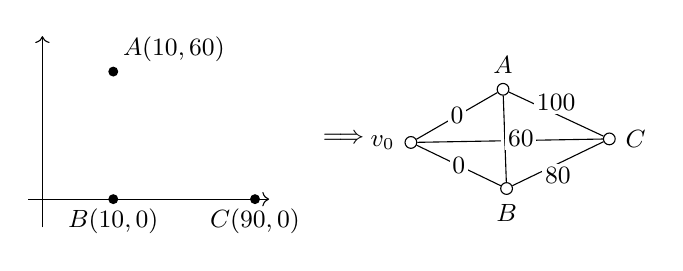
\begin{tikzpicture}[scale=0.9,every node/.style={font=\small}]
  \draw[->] (-0.2,0) -- (3.2,0);
  \draw[->] (0,-0.4) -- (0,2.3);
  \fill (1,1.8) circle (2pt) node[above right] {$A(10,60)$};
  \fill (1,0) circle (2pt) node[below] {$B(10,0)$};
  \fill (3,0) circle (2pt) node[below] {$C(90,0)$};
  \node at (4.25,0.85) {$\Longrightarrow$};
  \node[circle,draw,inner sep=1.5pt,label=left:$v_0$] (v0) at (5.2,0.8) {};
  \node[circle,draw,inner sep=1.5pt,label=above:$A$] (A) at (6.5,1.55) {};
  \node[circle,draw,inner sep=1.5pt,label=below:$B$] (B) at (6.55,0.15) {};
  \node[circle,draw,inner sep=1.5pt,label=right:$C$] (C) at (8.0,0.85) {};
  \foreach \p in {A,B,C} {
    \draw (v0)--(\p) node[midway,fill=white,inner sep=1pt] {$0$};
  }
  \draw (A)--(B) node[midway,right,fill=white,inner sep=1pt] {$60$};
  \draw (A)--(C) node[midway,above,fill=white,inner sep=1pt] {$100$};
  \draw (B)--(C) node[midway,below,fill=white,inner sep=1pt] {$80$};
\end{tikzpicture}
\caption{Ví dụ chuyển bài toán vệ tinh thành cây khung có ràng buộc bậc:
thêm đỉnh ảo $v_0$, nối nó với mọi làng bằng cạnh trọng số $0$, rồi yêu cầu
$d_T(v_0)=k$.}
\end{figure}

\subsection{Secret Milking Machine}

Farmer John cần vận chuyển sữa đến các điểm bán. Sữa có thể được chuyển trước
đến một vài điểm, rồi từ các điểm đó chuyển tiếp đến các điểm khác. Tổng
quãng đường càng nhỏ thì chi phí càng thấp, nhưng Farmer John không muốn đối
thủ biết phương án rẻ nhất, nên muốn dùng phương án có chi phí nhỏ thứ hai.

\begin{figure}[ht]
\centering
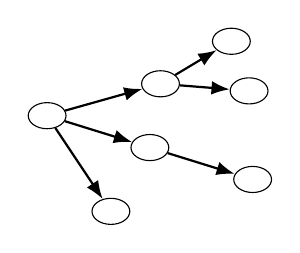
\begin{tikzpicture}[scale=0.9,>=Latex,every node/.style={font=\small}]
  \tikzset{p/.style={ellipse,draw,minimum width=0.48cm,minimum height=0.24cm}}
  \node[p] (s) at (0,0) {};
  \node[p] (a) at (1.6,0.45) {};
  \node[p] (b) at (1.45,-0.45) {};
  \node[p] (c) at (2.6,1.05) {};
  \node[p] (d) at (2.85,0.35) {};
  \node[p] (e) at (2.9,-0.9) {};
  \node[p] (f) at (0.9,-1.35) {};
  \draw[->,thick] (s)--(a);
  \draw[->,thick] (s)--(b);
  \draw[->,thick] (s)--(f);
  \draw[->,thick] (a)--(c);
  \draw[->,thick] (a)--(d);
  \draw[->,thick] (b)--(e);
\end{tikzpicture}
\caption{Một phương án vận chuyển có dạng cây: sữa có thể đi qua một số điểm
bán trước khi đến các điểm còn lại. Bài toán yêu cầu phương án cây có chi phí
nhỏ thứ hai.}
\end{figure}

Bài toán này là mô hình cây khung nhỏ thứ hai điển hình. Xem các điểm bán là
đỉnh của đồ thị, mỗi cặp điểm có một cạnh vô hướng có trọng số là khoảng cách
giữa chúng. Khi đó chỉ cần áp dụng thuật toán tìm cây khung nhỏ thứ hai đã
nêu ở trên.

\section{Kết luận}

Bài viết trình bày hai mở rộng của bài toán cây khung nhỏ nhất: cây khung có
ràng buộc bậc và cây khung nhỏ thứ hai. Trên thực tế, các mở rộng của cây
khung nhỏ nhất rất đa dạng, không chỉ gồm hai loại này; những mô hình kinh
điển khác trong tin học cũng tương tự. Khi giải bài toán thực tế, ta không nên
bị bó buộc vào mô hình kinh điển nguyên dạng, mà cần điều chỉnh và mở rộng mô
hình cho phù hợp đặc điểm của đề.

Điều đó không có nghĩa mô hình kinh điển đã lỗi thời. Mọi mở rộng đều dựa trên
mô hình gốc và có liên hệ chặt chẽ với nó. Vì vậy cần vừa nắm chắc các mô hình
kinh điển, vừa biết vận dụng linh hoạt và sáng tạo theo từng tình huống.

\section*{Tài liệu tham khảo}

\begin{enumerate}
  \item Xie Zheng, Li Jianping. \textit{Network Algorithms and Complexity
  Theory}.
  \item Yan Weimin, Wu Weimin. \textit{Data Structures}, 2nd edition.
  \item Thomas H. Cormen, Charles E. Leiserson, Ronald L. Rivest, Clifford
  Stein. \textit{Introduction to Algorithms}, 2nd edition.
\end{enumerate}

\end{document}
